\section{Utility Arrows}\label{utilfns}
Following are definitions of some utility Arrows used in this paper that have been left out for brevity.
We start with the |second| combinator from \citet{HughesArrows}, which is a mirrored version of |first|, which is for example used in the definition of |***|: 
\begin{code}
second :: Arrow arr => arr a b -> arr (c, a) (c, b)
second f = arr swap >>> first f >>> arr swap
	where swap (x, y) = (y, x)
\end{code}

Next, we give the definition of |evalN| which also helps us to define |map|, and |zipWith| on Arrows.
The |evalN| combinator in Fig.~\ref{fig:evalN} converts a list of arrows |[arr a b]| into an arrow |arr [a] [b]|.

\begin{figure}[h]
\begin{code}
evalN :: (ArrowChoice arr) => [arr a b] -> arr [a] [b]
evalN (f:fs) = arr listcase >>>
         arr (const []) ||| (f *** evalN fs >>> arr (uncurry (:)))
         where listcase []     = Left ()
               listcase (x:xs) = Right (x,xs)
evalN [] = arr (const [])
\end{code}
\caption{The definition of |evalN|}
\label{fig:evalN}
\end{figure}

The |mapArr| combinator (Fig.~\ref{fig:mapArr}) lifts any arrow |arr a
b| to an arrow |arr [a] [b]|. The original inspiration was from \cite{programming_with_arrows},
but the definition as then unified with |evalN|. 

\begin{figure}[h]
\begin{code}
mapArr :: ArrowChoice arr => arr a b -> arr [a] [b]
mapArr = evalN . repeat
\end{code}
\caption{The definition of |map| over Arrows.}
\label{fig:mapArr}
\end{figure}

Finally, with the help of |mapArr| (Fig.~\ref{fig:mapArr}), we can define |zipWithArr|  (Fig.~\ref{fig:zipWithArr}) that lifts any arrow |arr (a, b) c| to an arrow |arr ([a], [b]) [c]|.
\begin{figure}[h]
\begin{code}
zipWithArr :: ArrowChoice arr => arr (a, b) c -> arr ([a], [b]) [c]
zipWithArr f = (arr $ \(as, bs) -> zipWith (,) as bs) >>> mapArr f
\end{code}
\caption{|zipWith| over arrows.}
\label{fig:zipWithArr}
\end{figure}
 %$ %% formatting

These combinators make use of the |ArrowChoice| type class which provides the |pipepipepipe| combinator. It takes two arrows |arr a c| and |arr b c| and combines them into a new arrow |arr (Either a b) c| which pipes all |Left a|'s to the first arrow and all |Right b|'s to the second arrow:
% \begin{figure}[htb]
\begin{code}
(pipepipepipe) :: ArrowChoice arr a c -> arr b c -> arr (Either a b) c
\end{code}

\section{Profunctor Arrows}
\label{app:profunctorArrows}

In Fig.~\ref{fig:profunctorArrow} we show how specific Profunctors can be turned into Arrows. Note that in Standard GHC |(>>>)| has the type |(>>>) :: Category cat => cat a b -> cat b c -> cat a c| and is therefore not part of the |Arrow| typeclass.

\begin{figure}[h]
\begin{code}
instance (Category p, Strong p) => Arrow p where
  arr f = dimap id f id
  first = first'

instance (Category p, Strong p, Costrong p) => ArrowLoop p where
  loop = loop'

instance (Category p, Strong p, Choice p) => ArrowChoice p where
  left = left'
\end{code}
\caption{Profunctors as Arrows}
\footnote{for additional information on the typeclasses see: \url{https://hackage.haskell.org/package/profunctors-5.2.1/docs/Data-Profunctor.html} and \url{https://hackage.haskell.org/package/base-4.9.1.0/docs/Control-Category.html}}
\label{fig:profunctorArrow}
\end{figure}

\section{Omitted Function Definitions}
\label{app:omitted}
We have omitted some function definitions in the main text for
brevity, and redeem this here.


%
We begin with warping Eden's build-in |RemoteData| to |Future| in
Figure~\ref{fig:RDFuture}

\begin{figure}[h]
\begin{code}
data RemoteData a = RD { rd :: RD a }

put' :: (Arrow arr) => arr a (BasicFuture a)
put' = arr BF

get' :: (Arrow arr) => arr (BasicFuture a) a
get' = arr (\(~(BF a)) -> a)

instance NFData (RemoteData a) where
    rnf = rnf . rd
instance Trans (RemoteData a)

instance (Trans a) => Future RemoteData a Conf where
    put _ = put'
    get _ = get'

instance (Trans a) => Future RemoteData a () where
    put _ = put'
    get _ = get'
\end{code}
\caption{|RD|-based |RemoteData| version of |Future| for the Eden backend.}
\label{fig:RDFuture}
\end{figure}

Next, we have the definition of |BasicFuture| in Fig.~\ref{fig:BasicFuture} and the corresponding |Future| instances.

\begin{figure}[h]
\begin{code}
data BasicFuture a = BF a

put' :: (Arrow arr) => arr a (BasicFuture a)
put' = arr BF

get' :: (Arrow arr) => arr (BasicFuture a) a
get' = arr (\(~(BF a)) -> a)

instance NFData a => NFData (BasicFuture a) where
    rnf (BF a) = rnf a

instance Future BasicFuture a (Conf a) where
    put _ = put'
    get _ = get'

instance Future BasicFuture a () where
    put _ = put'
    get _ = get'
\end{code}
\caption{The |BasicFuture| type and its |Future| instance for the |Par| Monad and GpH Haskell backends.}
\label{fig:BasicFuture}
\end{figure}

% \caption{NFData and Trans instances for the RemoteData type. The Trans instance does not have any functions declared as the default implementation suffices here. See \url{https://hackage.haskell.org/package/edenmodules-1.2.0.0/docs/Control-Parallel-Eden.html\#g:5} for more information.}
% \end{figure}

Figures~\ref{fig:parMapImg}--\ref{fig:parMapStream} show the definitions and a visualizations of two parallel |map| variants, defined using |parEvalN| and its lazy counterpart.

\begin{figure}[thb]
%parMap
\includegraphics[scale=0.7]{images/parMap}
\caption{Schematic depiction of |parMap|.}
\label{fig:parMapImg}

\begin{code}
parMap :: (ArrowParallel arr a b conf) => conf -> (arr a b) -> (arr [a] [b])
parMap conf f = parEvalN conf (repeat f)
\end{code}
\caption{Definition of parMap.}
\label{fig:parMap}

%parMapStream
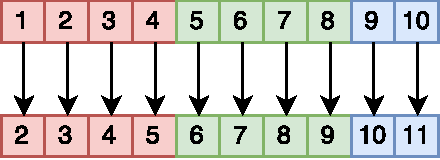
\includegraphics[scale=0.7]{images/parMapStream}
\caption{Schematic depiction of |parMapStream|.}
\label{fig:parMapStreamImg}

\begin{code}
parMapStream :: (ArrowParallel arr a b conf, ArrowChoice arr, ArrowApply arr) =>
	conf -> ChunkSize -> arr a b -> arr [a] [b]
parMapStream conf chunkSize f = parEvalNLazy conf chunkSize (repeat f)
\end{code}
\caption{Definition of |parMapStream|.}
\label{fig:parMapStream}
\end{figure}

Arrow versions of Eden's |shuffle|, |unshuffle| and the definition of |takeEach| are in Figure~\ref{fig:edenshuffleetc}. Similarly, Figure~\ref{fig:edenlazyrightrotate} contains the definition of arrow versions of Eden's |lazy| and |rightRotate| utility functions. Fig.~\ref{fig:lazyzip3etc} contains Eden's definition of |lazyzip3| together with the utility functions |uncurry3| and |threetotwo|.
The full definition of |farmChunk| is in Figure~\ref{fig:farmChunk}.
Eden definition of |ring| skeleton is in Figure~\ref{fig:ringEden}. It
follows \citet{Loogen2012}.

\begin{figure}[h]
\begin{code}
shuffle :: (Arrow arr) => arr [[a]] [a]
shuffle = arr (concat . transpose)

unshuffle :: (Arrow arr) => Int -> arr [a] [[a]]
unshuffle n = arr (\xs -> [takeEach n (drop i xs) | i <- [0..n-1]])

takeEach :: Int -> [a] -> [a]
takeEach n [] = []
takeEach n (x:xs) = x : takeEach n (drop (n-1) xs)
\end{code}
\caption{Definitions of |shuffle|, |unshuffle|, |takeEach|.}
\label{fig:edenshuffleetc}
\end{figure}

\begin{figure}[h]
\begin{code}
lazy :: (Arrow arr) => arr [a] [a]
lazy = arr (\ ~(x:xs) -> x : lazy xs)

rightRotate :: (Arrow arr) => arr [a] [a]
rightRotate = arr $ \list -> case list of
  [] -> []
  xs -> last xs : init xs
\end{code}
\caption{Definitions of |lazy| and |rightRotate|.}
\label{fig:edenlazyrightrotate}
\end{figure}

\begin{figure}[h]
\begin{code}
lazyzip3 :: [a] -> [b] -> [c] -> [(a, b, c)]
lazyzip3 as bs cs = zip3 as (lazy bs) (lazy cs)

uncurry3 :: (a -> b -> c -> d) -> (a, (b, c)) -> d
uncurry3 f (a, (b, c)) = f a b c

threetotwo :: (Arrow arr) => arr (a, b, c) (a, (b, c))
threetotwo = arr $ \ ~(a, b, c) -> (a, (b, c))
\end{code}
\caption{Definitions of |lazyzip3|, |uncurry3| and |threetotwo|.}
\label{fig:lazyzip3etc}
\end{figure}

\begin{figure}[h]
\begin{code}
farmChunk :: (ArrowParallel arr a b conf, ArrowParallel arr [a] [b] conf, 
             ArrowChoice arr, ArrowApply arr) =>
	conf -> ChunkSize -> NumCores -> arr a b -> arr [a] [b]
farmChunk conf chunkSize numCores f =
	unshuffle numCores >>>
	parEvalNLazy conf chunkSize (repeat (mapArr f)) >>>
	shuffle
\end{code}
\caption{Definition of |farmChunk|.}
\label{fig:farmChunk}
\end{figure}

\begin{figure}[h]
\begin{code}
ringSimple :: (Trans i, Trans o, Trans r) => (i -> r -> (o,r)) -> [i] -> [o]
ringSimple f is =  os
  where (os,ringOuts) = unzip (parMap (toRD $ uncurry f) (zip is $ lazy ringIns))
        ringIns = rightRotate ringOuts

toRD :: (Trans i, Trans o, Trans r) => ((i,r) -> (o,r)) -> ((i, RD r) -> (o, RD r))
toRD  f (i, ringIn)  = (o, release ringOut)
  where (o, ringOut) = f (i, fetch ringIn)

rightRotate    :: [a] -> [a]
rightRotate [] =  []
rightRotate xs =  last xs : init xs

lazy :: [a] -> [a]
lazy ~(x:xs) = x : lazy xs
\end{code}
\caption{Eden's definition of the |ring| skeleton.}
\label{fig:ringEden}
\end{figure}

The |parEval2| skeleton is defined in Figure~\ref{fig:parEval2}. 
We start by transforming the |(a, c)| input into a two-element list |[Either a c]| by first tagging the two inputs with |Left| and |Right| and wrapping the right element in a singleton list with |return| so that we can combine them with |arr (uncurry (:))|. Next, we feed this list into a parallel arrow running on two instances of |f +++ g| as described above. After the calculation is finished, we convert the resulting |[Either b d]| into |([b], [d])| with |arr partitionEithers|. The two lists in this tuple contain only one element each by construction, so we can finally just convert the tuple to |(b, d)| in the last step.
\begin{figure}[h]
\begin{code}
parEval2 :: (ArrowChoice arr,
	ArrowParallel arr (Either a c) (Either b d) conf) =>
	conf -> arr a b -> arr c d -> arr (a, c) (b, d)
parEval2 conf f g =
	arr Left *** (arr Right >>> arr return) >>>
	arr (uncurry (:)) >>>
	parEvalN conf (replicate 2 (f +++ g)) >>>
	arr partitionEithers >>>
	arr head *** arr head
\end{code}
	\caption{Definition of |parEval2|.}
	\label{fig:parEval2}
\end{figure}
Furthermore, Fig.~\ref{fig:torus_example_rest} contains the omitted definitions of |prMMTr| (which calculates $AB^T$ for two matrices $A$ and $B$), |splitMatrix| (which splits the a matrix into chunks), and lastly |matAdd|, that calculates $A + B$ for two matrices $A$ and $B$.
\begin{figure}[h]
\begin{code}
prMMTr m1 m2 = [[sum (zipWith (*) row col) | col <- m2 ] | row <- m1]

splitMatrix :: Int -> Matrix -> [[Matrix]]
splitMatrix size matrix = map (transpose . map (chunksOf size)) $ chunksOf size $ matrix

matAdd = chunksOf (dimX x) $ zipWith (+) (concat x) (concat y)
\end{code}
	\caption{Definition of |prMMTr|, |splitMatrix| and |matAdd|.}
	\label{fig:torus_example_rest}
\end{figure}

\section{Syntactic Sugar} \label{syntacticSugar}
Finally, we also give the definitions for some syntactic sugar for PArrows, namely |***| and |&&&|.
For basic arrows, we have the |***| combinator (Fig.~\ref{fig:syntacticSugarArrows}) which allows us to combine two arrows |arr a b| and |arr c d| into an arrow |arr (a, c) (b, d)| which does both computations at once. This can easily be translated into a parallel version |***| with the use of |parEval2|, but for this we require a backend which has an implementation that does not require any configuration (hence the |()| as the |conf| parameter% in Fig.~\ref{fig:par***}
):
% \begin{figure}[h]
\begin{code}
(|***|) :: (ArrowChoice arr, ArrowParallel arr (Either a c) (Either b d) ())) =>
	arr a b -> arr c d -> arr (a, c) (b, d)
(|***|) = parEval2 ()
\end{code}
% \caption{Definition of |parstar|, the parallel version of |***|.}
% \label{fig:par***}
% \end{figure}
% With this we can analogously to the serial |&&&|
We define the parallel |&&&| % (Fig.~\ref{fig:par&&&}) 
in a similar manner to its sequential pendant |&&&| (Fig.~\ref{fig:syntacticSugarArrows}):
% \begin{figure}[h]
\begin{code}
(|&&&|) :: (ArrowChoice arr, ArrowParallel arr (Either a a) (Either b c) ()) =>
	arr a b -> arr a c -> arr a (b, c)
(|&&&|) f g = (arr $ \a -> (a, a)) >>> f |***| g
\end{code} % $ %% formatting
% \caption{Definition of |parand| - the parallel version of |&&&|.}
% \label{fig:par&&&}
% \end{figure}


%%% Local Variables:
%%% mode: latex
%%% TeX-master: "main"
%%% End:
